\documentclass{beamer}
\usefonttheme[onlymath]{serif}
\usepackage[orientation=portrait,size=a0,scale=1.4,debug]{beamerposter}
\mode<presentation>{\usetheme{ZH}}
\usepackage{chemformula}
\usepackage[utf8]{inputenc}
\usepackage[T1]{fontenc}
\usepackage[czech]{babel} 
\usepackage{siunitx} %pretty measurement unit rendering
\usepackage{hyperref} %enable hyperlink for urls
\usepackage{ragged2e}
\usepackage[font=scriptsize,justification=justified, figurename=Obr., tablename=Tab.]{caption}
\usepackage{array,booktabs,tabularx}
\usepackage[version=4]{mhchem}
\usepackage{lmodern}
\usepackage{exscale}
\usepackage{siunitx}
\sisetup{output-decimal-marker = {,}}
\sisetup{separate-uncertainty}
\usepackage{collcell}
\usepackage{microtype}
\usepackage{multirow}
\usepackage{amsmath}
\usepackage{amsfonts}
\usepackage{amssymb}
\usepackage{subcaption}
\usepackage{scrextend}
\usepackage{textcomp}
\usepackage{wrapfig}

\newcolumntype{Z}{>{\centering\arraybackslash}X} % centered tabularx columns
\sisetup{per=frac,fraction=sfrac}

\title{\huge Multi-kompártmentový přístup ke kvantifikaci a lokalizaci přísunů radonu do budov s využitím techniky indikačních plynů}
\author[michal.sestak@suro.cz]{Michal Šesták$^{1,2}$, Karel Jílek$^{1}$}
%\institute[ETH]{$^{1}$Institute for Biomedical Engineering, ETH and University of Zurich \\ $^{2}$Preclinical Laboratory for Translational Research into Affective Disorders, DPPP, Psychiatric Hospital, University of Zurich}
\institute[SÚRO]{$^{1}$Státní ústav radiační ochrany, v. v. i. \\ $^{2}$Fakulta jaderná a fyzikálně inženýrská, ČVUT v Praze}
\date{5. listopadu 2019}

% edit this depending on how tall your header is. We should make this scaling automatic :-/
\newlength{\columnheight}
%\setlength{\columnheight}{104cm}
\setlength{\columnheight}{99cm}

\begin{document}
\shorthandoff{-}
\begin{frame}
\begin{columns}
	\begin{column}{.43\textwidth}
		\begin{beamercolorbox}[center]{postercolumn}
			\begin{minipage}{.98\textwidth}  % tweaks the width, makes a new \textwidth
				\parbox[t][\columnheight]{\textwidth}{ % must be some better way to set the the height, width and textwidth simultaneously
\begin{myblock}{Úvod}
    \begin{columns}
        \begin{column}{.6\textwidth}
            %\begin{labeling}{\textbf{Provedení}}
            \begin{description}
            \item[\textbf{Motivace}] radonová diagnostika budov s využitím techniky indikačních plynů 
            \item[\textbf{Cíl}] vytvoření výpočetního modelu pro lokalizaci a kvantifikaci přísunů radonu do jednotlivých částí objektu a jeho ověření na naměřených datech; dále vytipovat nejvhodnější kombinaci indikačních plynů
            \item[\textbf{Postup}]\mbox{}
                \begin{enumerate}
                    \item rozdělení objektu na kompártmenty (zóny)
                    \item potřeba znát obj. průtoky vzduchu mezi kompartmenty \textrightarrow{} metoda indikačních plynů
                    %\item potřeba znát průměrné OAR v kompártmentech \textrightarrow{} TESLA TSR sondy \& CANARY detektory
                    %\item potřeba znát objemy kompártmentů
                    %\item výpočet pomocí soustavy rovnic~\eqref{eq:vypocet}
                \end{enumerate}
            %\item[\textbf{Ověření}] proměřily se tři objekty (viz tab.~\ref{tab:prehled}) s definovanými přísuny radonu do kompártmentů

            \end{description}
                %, v případě vícepodlažních budov většinou podle podlaží, 
        \end{column}
        \begin{column}{.4\textwidth}
            \begin{figure}[h]
                \centering
                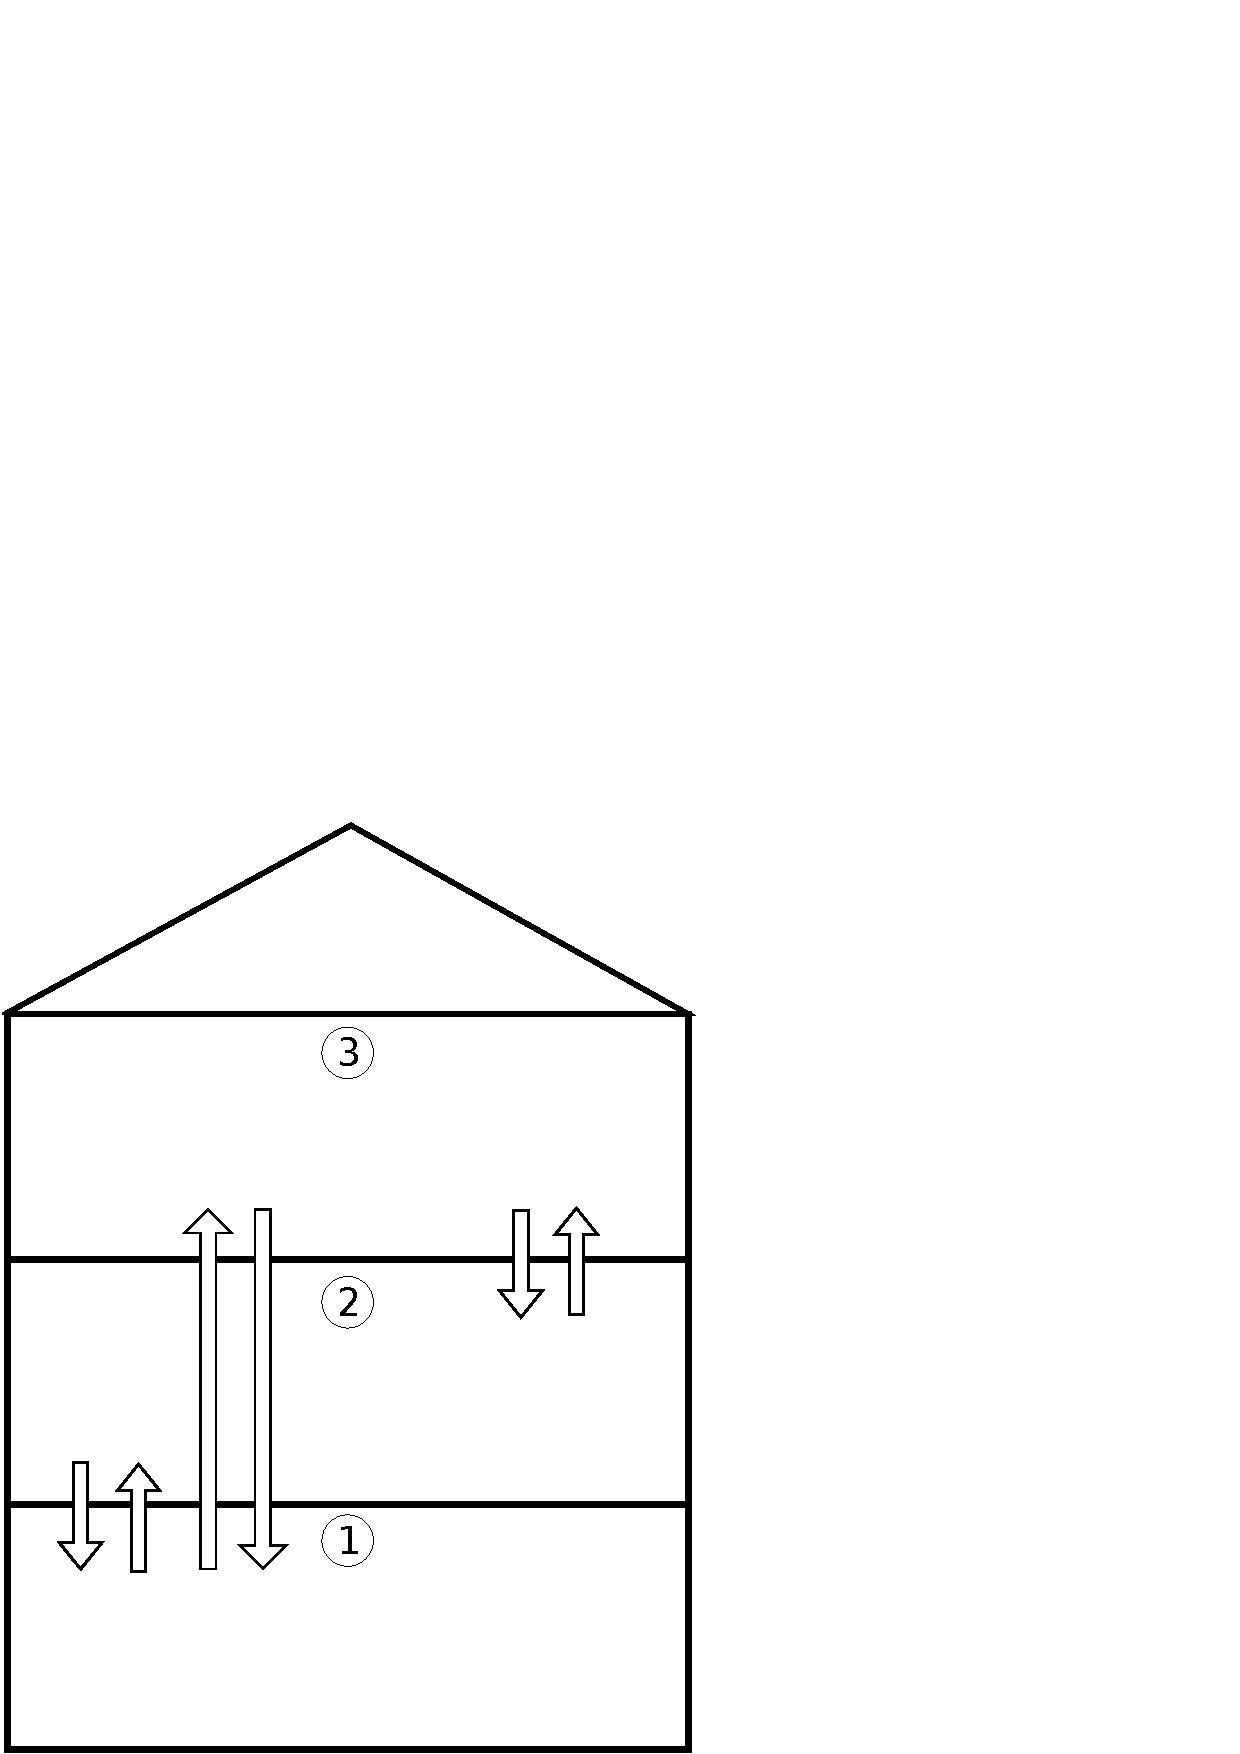
\includegraphics[width=\textwidth]{podklady/obrys_domu.pdf}
                \caption{Obrys třípodlažního domu, každé podlaží představuje kompartment. Značení veličin viz tab.~\ref{tab:veliciny}.}
                \label{fig:princip}
            \end{figure}
        \end{column}
    \end{columns}

    \vspace{7pt}
    \begin{enumerate}\setcounter{enumi}{2}
        {\setlength\itemindent{25pt}\item potřeba znát průměrné OAR v kompártmentech \textrightarrow{} TESLA TSR sondy \& CANARY měřidla}
    {\setlength\itemindent{25pt}\item potřeba znát objemy kompártmentů}
    {\setlength\itemindent{25pt}\item výpočet pomocí soustavy rovnic~\eqref{eq:vypocet}}
    {\setlength\itemindent{25pt}\item použití průtokových zdrojů radonu typu RF 2000 (ČMI Praha) pro realizaci známých přísunů radonu}
    \end{enumerate}
    \begin{description}
            \item[\textbf{Ověření modelu}] pro ilustraci byly vybrány výsledky z dvou objektů (viz tab.~\ref{tab:prehled}) s definovanými přísuny radonu do kompártmentů
    \end{description}
\begin{table}
    \scriptsize
    \centering
    \caption{Objekty, v nichž bylo provedeno měření přísunů radonu. $N$ je počet kompartmentů, na který byl daný objekt rozdělen.}
    \label{tab:prehled}
    	\begin{tabular}{lllll}
		\toprule
		Objekt & Rozsah měření & $t$ [dny] & Typ objektu &$N$\\
		\midrule
		Skála 75, okr. Havlíčkův Brod & 23. 5. -- 5. 6. 2019 & 14 & chata & 3\\
		Hálková 980, Humpolec & 5. 6. -- 20. 6. 2019 & 15 & byt & 4\\
		Anglická 574, Dobřichovice & 9. 7. -- 30. 7. 2019 & 22 & rodinný dům & 3\\
		\bottomrule
	\end{tabular}

\end{table}
\end{myblock}\vfill


\begin{myblock}{Metoda indikačních plynů}
    %\begin{columns}
        %\begin{column}{.55\textwidth}
            \begin{itemize}
                \item integrální technika (popsána v~\cite{metodika})
                \item podmínka $N_p\geq N$, kde $N_p$ je počet indikačních plynů a $N$ počet zón
                \item \textbf{doba měření:} 14 až 31 dní
                \item vyhodnocení pomocí plynového chromatografu s termální desorpcí
                \item \textbf{výsledek:} obj. průtoky vzduchu mezi kompártmenty, exfiltrace vzduchu z kompártmentů a výměna vzduchu budovy
            \end{itemize} 
            \vspace{1em}
    \begin{minipage}{.5\textwidth}
        \begin{figure}
            \centering
            \includegraphics[width=.9\textwidth]{podklady/vyvijec_TDdetektory.jpg}
            \caption{Vyvíječe a TD detektory.}
            \label{fig:vyvijec}
        \end{figure}
    \end{minipage}
    \begin{minipage}{.5\textwidth}
        \begin{figure}
            \centering
            \includegraphics[width=.85\textwidth]{podklady/transport_bedna.jpg}
            \caption{Transportní bedna pro vyvíječe a TD detektory.}
            \label{fig:transport}
        \end{figure}
    \end{minipage}
\end{myblock}\vfill

\begin{myblock}{Výpočetní model}

\begin{itemize}
    \item výpočet infiltrací:
        \begin{equation}
            k_{i_I}=k_{i_E}+\sum_{j=1}^{N} \left(k_{ij}-k_{ji}\right)
            \label{eq:infiltrace}
        \end{equation}
    \item soustava rovnic popisující systém:
        \begin{equation}
            0=\frac{1}{V_i}\left( \sum^{N+1}_{j=1}\overline{a_j} k_{ji}-\sum^{N+1}_{j=1}\overline{a_i} k_{ij}\right)-\lambda \overline{a_i} +\overline{Q_i}\,,\quad i\in \{1,2,\ldots,N\}\label{eq:vypocet}
        \end{equation}
\end{itemize}

\begin{table}[h]
\def\arraystretch{1.1}
\scriptsize
    \centering
    \caption{Značení a jednotky používaných veličin.}
    \label{tab:veliciny}
    \begin{tabular}{lp{.7\textwidth}l}
    %\begin{tabular}{lll}
        \toprule
        $N$   & počet kompartmentů/zón uvnitř zkoumaného objektu&[-]\\
        $V_i$ & objem $i$-té zóny& [\si{m^3}] \\
        $k_{ij}$ & objemový průtok vzduchu z $i$-té zóny do $j$-té zóny& [\si{m^3/hod}]\\
        $k_{i, N+1}$ & exfiltrace $i$-té zóny, ozn. $k_{i_E}$; index $N+1$ značí vnější prostředí & [\si{m^3/hod}]\\
        $k_{N+1, i}$ & infiltrace $i$-té zóny, ozn. $k_{i_I}$; index $N+1$ značí vnější prostředí &[\si{m^3/hod}]\\
        $a_i$ & OAR v $i$-té zóně& [\si{Bq/m^3}] \\
        $\lambda$ & přeměnová konstanta radonu& [\si{1/hod}]\\
        $Q_i$ & přísun radonu do $i$-té zóny& $\left[\si{\frac{Bq}{m^3\cdot hod}}\right]$ \\
        \bottomrule
    \end{tabular}
\end{table}
\end{myblock}\vfill

		}\end{minipage}\end{beamercolorbox}
	\end{column}



	\begin{column}{.57\textwidth}
		\begin{beamercolorbox}[center]{postercolumn}
			\begin{minipage}{.98\textwidth} % tweaks the width, makes a new \textwidth
				\parbox[t][\columnheight]{\textwidth}{ % must be some better way to set the the height, width and textwidth simultaneously


\begin{myblock}{Výsledky z objektu 1}
    \begin{columns}
        \centering
        \begin{column}{.55\textwidth}
            \begin{figure}
                \centering
                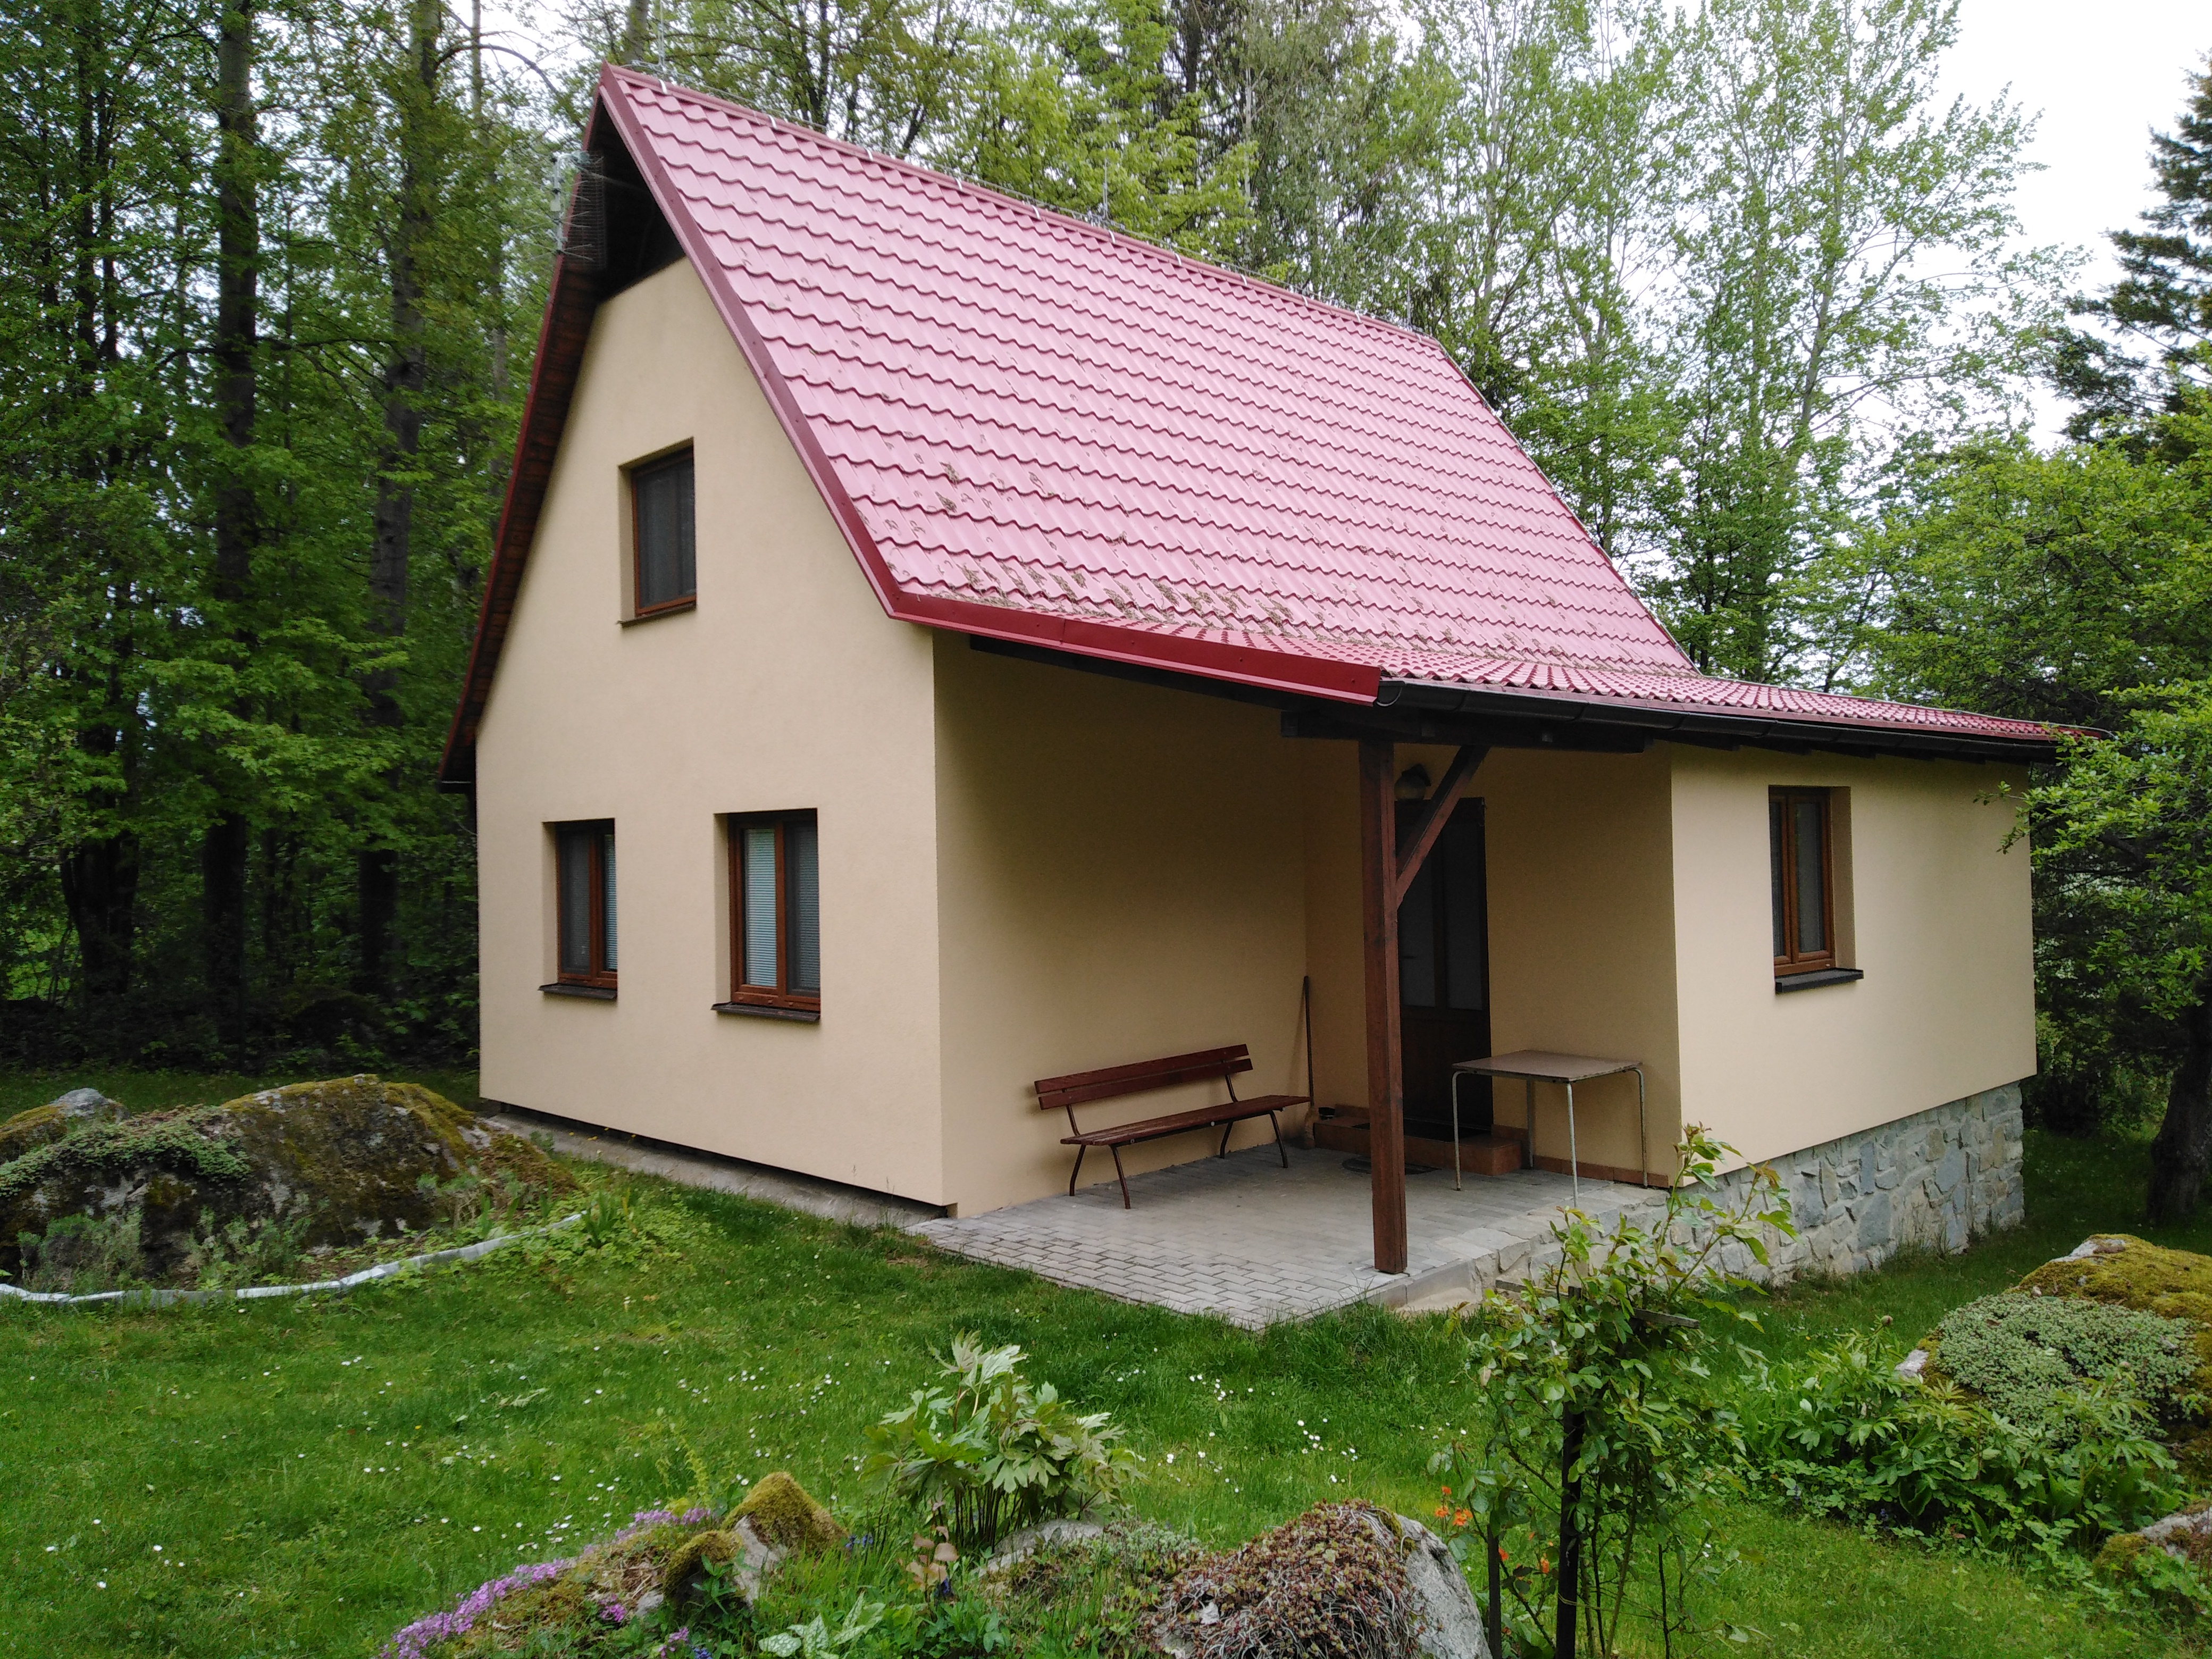
\includegraphics[width=.7\textwidth]{podklady/humpolec_chata.jpg}
                \label{fig:skala75_dum}
            \end{figure}
            \begin{itemize}
                \item $N=3$ (sklep, přízemí, první patro)
                \item 14 vyvíječů, 12 TD detektorů, 3 teploměry
                \item 6 typů tracerů (TMH, MCH, PCH a MDC jsou fluorované uhlovodíky, TCE a PCE jsou chlorované uhlovodíky)
                \item 2 průtočné zdroje radonu (umístěny do sklepa a do kuchyně v přízemí)
                \item 4 TESLA TSR sondy, 4 CANARY měřidla
            \end{itemize}
            Dvojnásobné množství použitých tracerů oproti počtu zón umožnilo vyhodnotit data osmi způsoby.
            \begin{itemize}
                \item výměna vzduchu v rozmezí 0,2 až 0,3 \si{hod^{-1}}
            \end{itemize}
            \begin{table}
                \scriptsize
                \centering
                \caption{Průměrné OAR [\si{Bq/m^3}] naměřené TESLA TSR sondami a CANARY měřidly.}
                \label{tab:skala75_OAR}
                \begin{tabular}{lrr}
\toprule
podlaží & TESLA TSR & CANARY \\
\midrule
sklep          & $458\pm33$ & $381\pm38$\\
přízemí kuchyň & $789\pm43$ & $419\pm42$\\
přízemí ložnice& $633\pm37$ & $465\pm47$\\
první patro    & $276\pm31$ & $156\pm16$\\
\bottomrule
\end{tabular}

            \end{table}
        \end{column}
            %\begin{table}
                %\centering
                %\scriptsize
                %\caption{Obj. průtoky vzduchu a výměna vzduchu $n$ pro třetí a pátou kombinaci indikačních plynů (z celkového počtu osmi kombinací).}
                %\label{tab:skala75_prutoky}
                %\begin{tabular}{l>{\raggedleft\arraybackslash}p{4cm}>{\raggedleft\arraybackslash}p{4cm}}
\toprule
& (TMH, MCH, PCE)               & (TCE, MDC, PCE)\\
\midrule                                                
$k_{12}$ &  10,188$\pm$2,611    & 7,859$\pm$1,288\\
$k_{13}$ &   0,908$\pm$0,261    & 0,893$\pm$0,159\\
$k_{21}$ &   3,220$\pm$0,776    & 1,309$\pm$0,211\\
$k_{23}$ &   1,025$\pm$0,161    & 1,235$\pm$0,180\\
$k_{31}$ &  -0,061$\pm$0,016    &-0,025$\pm$0,005\\
$k_{32}$ &   0,774$\pm$0,117    & 0,922$\pm$0,136\\
&&\\                                           
$k_{1_E}$&  23,244$\pm$5,443    & 2,474$\pm$1,325\\
$k_{2_E}$&  36,712$\pm$4,240    &46,234$\pm$4,862\\
$k_{3_E}$&   7,850$\pm$0,853    & 7,670$\pm$0,848\\
$k_{1_I}$&  31,181$\pm$6,093    & 9,941$\pm$1,867\\
$k_{2_I}$&  29,994$\pm$5,043    &39,997$\pm$5,039\\
$k_{3_I}$&   6,630$\pm$0,914    & 6,439$\pm$0,891\\
\midrule                                         
$n$      &   0,287$\pm$0,036    & 0,239$\pm$0,028\\
\bottomrule
\end{tabular}

            %\end{table}

        %\end{column}
    %\end{columns}
    \begin{column}{.45\textwidth}
    \begin{figure}
        \centering
        \includegraphics[width=\textwidth]{podklady/prisuny_grafy/skala75_errorbar.png}
        \caption{Srovnání určených přísunů radonu do kompártmentů se známými přísuny radonu ze zdrojů. Pro výpočet byly použity OAR z TERA sond.}
        \label{fig:skala75_prisuny_sondy}
    \end{figure}
    \begin{figure}
        \centering
        \includegraphics[width=\textwidth]{podklady/prisuny_grafy/skala75_CANARY_errorbar.png}
        \caption{To samé jako v obr.~\ref{fig:skala75_prisuny_sondy}, kdy byly pro výpočet použity OAR z CANARY měřidel.}
    \end{figure}
\end{column}
\end{columns}
    %\begin{minipage}{.8\textwidth}
        %\begin{table}
            %\scriptsize
            %\centering
            %\caption{Vypočítané přísuny radonu při použití OAR z: (a) TESLA TSR sond, (b) CANARY detektorů. V posledním řádku jsou uvedeny známé přísuny radonu z průtočných zdrojů.}
            %\label{tab:skala75_Q}
            %\begin{subtable}{0.45\textwidth}
                %\centering
                %\caption{}
                %\label{tab:skala75_Q_sondy}
                %\input{tabs/standalone_Q_sondy.tex}
            %\end{subtable}
            %\begin{subtable}{0.45\textwidth}
                %\centering
                %\caption{}
                %\label{tab:skala75_Q_CANARY}
                %\input{tabs/standalone_Q_CANARY.tex}
            %\end{subtable}
        %\end{table}
    %\end{minipage}

\end{myblock}\vfill


\begin{myblock}{Výsledky z objektu 2}
%\begin{columns}
    %\begin{column}{.6\textwidth}
    \begin{itemize}
        \item $N=3$ (sklep, přízemí, první patro)
        \item 2 zdroje radonu, oba dva umístěny do sklepa
        %\item 3 typy tracerů
        \item ve sklepě byla naměřena OAR~$=\SI{2800(200)}{Bq/m^3}$ \textrightarrow{} podezření na nenulový přirozený přísun radonu do sklepa \textrightarrow{} proběhlo dodatečné měření OAR ve sklepě bez zdrojů
        \item ukázalo se, že v závislosti na počasí se OAR ve sklepě pohybuje mezi 350 až 1700 \si{Bq/m^3}
        \item ze zpětného ověření se zjistilo, že přísunu radonu ze zdroje odpovídá OAR ve sklepě \SI{1200(400)}{Bq/m^3}
        \item výměna vzduchu $=\SI{0.29(4)}{hod^{-1}}$
    \end{itemize}
    %\end{column}
    %\begin{column}{.4\textwidth}
        %\begin{figure}
            %\centering
            %\includegraphics[width=\textwidth]{podklady/prisuny_grafy/halkova980_CANARY_errorbar.png}
            %\caption{Srovnání určených přísunů radonu se známými hodnotami pro objekt Hálková 980. OAR bylo bráno z CANARY detektorů.}
            %\label{fig:prisuny_halkova980}
        %\end{figure}
        %\begin{figure}
            %\centering
            %\includegraphics[width=\textwidth]{podklady/prisuny_grafy/anglicka574_CANARY_errorbar.png}
            %\caption{Srovnání určených přísunů radonu se známými hodnotami pro objekt 2. OAR bylo bráno z CANARY měřidel.}
            %\label{fig:prisuny_anglicka574}
        %\end{figure}
        \begin{table}
            \centering
            \scriptsize
            \caption{Srovnání určených přísunů radonu se známými přísuny radonu ze zdrojů, [$Q_i$]=\si{Bq/m^3/hod}.}
            \label{tab:prisuny_anglicka574}
            \begin{tabular}{lr@{${}\pm{}$}rr@{${}\pm{}$}rr@{${}\pm{}$}r}
        \toprule
        &\multicolumn{2}{r}{$Q_1$} & \multicolumn{2}{r}{$Q_2$}  & \multicolumn{2}{r}{$Q_3$} \\
        \midrule
(MCH, MDC, PCH) & 1057&245 & $-$31&13 & 21&7\\
        \midrule
zdroje & 455&90 & 0&0 & 0&0\\
        \bottomrule
    \end{tabular}

        \end{table}
    %\end{column}
%\end{columns}
\end{myblock}\vfill

\begin{myblock}{Závěr}
    Byl odvozen výpočetní model a dosažené výsledky potvrzují jeho použitelnost. Z výsledků měření prvního objektu byla nalezena nejvhodnější kombinace indikačních plynů (TMH, MCH, PCE). Z porovnání výsledků použitých dvou typů měřidel (CANARY, TESLA TSR) vyplynula lepší použitelnost výsledků z CANARY. Pro tuto kombinaci indikačních plynů byl nalezen relativní rozdíl mezi určenými hodnotami přísunů radonu stanovenými pomocí monitorů CANARY a známými hodnotami stanovenými pomocí použitých umělých průtokových zdrojů radonu typu RF 2000 menší než 20 \%.

U druhého objektu byla nalezena větší relativní diskrepance mezi naměřenými a známými hodnotami větší než u prvního objektu z důvodu později nalezeného přirozeného vysokého přísunu radonu do objektu.
    %U druhého objektu nesouhlasí určený přísun radonu do sklepa se známou hodnotou, což je dáno velikým přirozeným přísunem radonu, který nebyl zprvu uvažován. Z toho plyne větší relativní diskrepance mezi určenými a známými hodnotami.
    %Proběhlo dodatečné měření s cílem zjistit přirozenou OAR ve sklepu

Metoda bude dále vyvíjena a testována.
\end{myblock}
\vfill
\begin{myblock}{Reference}
    \footnotesize
    \tiny
    \begin{thebibliography}{Mn99}
                                \bibitem{japonci2} OKUYAMA, Hiroyasu, Yoshinori ONISHI, Shin-ichi TANABE a Seiichi KASHIHARA. Statistical data analysis method for multi-zonal airflow measurement using multiple kinds of perfluorocarbon tracer gas. Building and Environment [online]. 2009, 44(3), 546-557. DOI: 10.1016/j.buildenv.2008.04.014. ISSN 03601323. Dostupné z: \url{https://linkinghub.elsevier.com/retrieve/pii/S0360132308000905} 
                                \bibitem{sherman} SHERMAN, Max H., Iain S. WALKER a Melissa M. LUNDEN. Uncertainties in Air Exchange using Continuous-Injection, Long-Term Sampling Tracer-Gas Methods. International Journal of Ventilation [online]. 2016, 13(1), 13-28. DOI: 10.1080/14733315.2014.11684034. ISSN 1473-3315. Dostupné z: \url{http://www.tandfonline.com/doi/full/10.1080/14733315.2014.11684034}
                                \bibitem{metodika} JÍLEK, Karel; FROŇKA, Aleš. Metodika stanovení výměny vzduchu ve vnitřním ovzduší budov s využitím pasivních integrálních měřidel indikačních plynů (pro potřeby SÚJB) [online]. 2016 [cit. 2019-08-01]. Dostupné z: \url{https://www.sujb.cz/
fileadmin/sujb/docs/dokumenty/metodiky/Stanoveni_vymeny_vzduchu.pdf.}
                        \end{thebibliography}
                    \end{myblock}\vfill
		}\end{minipage}\end{beamercolorbox}
	\end{column}
\end{columns}

%\begin{myblock}{Reference}
    %\footnotesize
    %\tiny
    %\begin{thebibliography}{Mn99}
                                %\bibitem{japonci2} OKUYAMA, Hiroyasu, Yoshinori ONISHI, Shin-ichi TANABE a Seiichi KASHIHARA. Statistical data analysis method for multi-zonal airflow measurement using multiple kinds of perfluorocarbon tracer gas. Building and Environment [online]. 2009, 44(3), 546-557. DOI: 10.1016/j.buildenv.2008.04.014. ISSN 03601323. Dostupné z: \url{https://linkinghub.elsevier.com/retrieve/pii/S0360132308000905} 
                                %\bibitem{metodika} JÍLEK, Karel; FROŇKA, Aleš. Metodika stanovení výměny vzduchu ve vnitřním ovzduší budov s využitím pasivních integrálních měřidel indikačních plynů (pro potřeby SÚJB) [online]. 2016 [cit. 2019-08-01]. Dostupné z: \url{https://www.sujb.cz/
%fileadmin/sujb/docs/dokumenty/metodiky/Stanoveni_vymeny_vzduchu.pdf.}
                                %%\bibitem{sherman} SHERMAN, Max H., Iain S. WALKER a Melissa M. LUNDEN. Uncertainties in Air Exchange using Continuous-Injection, Long-Term Sampling Tracer-Gas Methods. International Journal of Ventilation [online]. 2016, 13(1), 13-28. DOI: 10.1080/14733315.2014.11684034. ISSN 1473-3315. Dostupné z: \url{http://www.tandfonline.com/doi/full/10.1080/14733315.2014.11684034}
                        %\end{thebibliography}
                    %\end{myblock}\vfill
\end{frame}
\end{document}
